\documentclass[../Main.tex]{subfiles}% Vietnam green
\begin{document}
	\section{World UBIs Quantitative Data}
	To establish a global context for the UBI landscape and to provide comparative quantitative insights, data on UBIs worldwide will be collected from reputable international reports, surveys, and academic studies. This macro-level data will inform the understanding of general trends, common characteristics, and the overall impact of UBIs globally, serving as a benchmark for the subsequent analysis of Vietnam-specific data.
	
	\subsection{Prevalence and Scope of University-Based Programs}
	The landscape of University-Based Incubation Programs (UBIs) globally is dynamic, with UBI Global's World Benchmark Studies and Community Reports providing comprehensive insights into its evolution.
	
	The \textbf{2019-2020 UBI Global World Benchmark Study} initially assessed a total of \textbf{1,580 programs}, with \textbf{364 programs} from \textbf{82 countries} retained for its rigorous benchmarking process \cite{ubi2019world}. This study highlighted a significant and widespread presence of business incubation and acceleration initiatives across six global regions. Within this sample, \textbf{41\%} were classified as "World Top University Business Incubators" and \textbf{10\%} as "World Top University Business Accelerators," indicating a substantial representation and high performance of university-linked programs globally \cite{ubi2019world}.
	
	The \textbf{2021-2022 UBI Global World Benchmark Study} shows a shift in the study's scope, reflecting a more focused assessment. This later study included \textbf{109 business incubators and accelerators} located in \textbf{56 countries} \cite{ubi2021world}.
	
	The \textbf{2023 UBI Global Community Report} demonstrates the continued expansion and diversity of the global ecosystem, with \textbf{over 1,000 business accelerators and incubators in more than 90 countries} as of March 2023. This broader community includes a wide range of program types, sector focuses, and regional participation, further highlighting the global reach and impact of university-based and other incubation programs \cite{Amin2024Incubators}.
	
	\begin{figure}[h]
		\centering
		\begin{tikzpicture}[
			node distance=1cm,
			box/.style={rectangle, draw, rounded corners, minimum width=2.5cm, minimum height=1cm, align=center, font=\small},
			arrow/.style={->, thick},
			percentage/.style={rectangle, draw, fill=blue!20, rounded corners, minimum width=3cm, align=center, font=\small, text width=3cm}
		]
		
		% Nodes
		\node[box, fill=green!20] (initial) {Initial Assessment\\1,580 programs\\82 countries};
		
		\node[box, fill=yellow!20, right=2.5cm of initial] (filter) {Rigorous Benchmarking\\Process};
		
		\node[box, fill=orange!20, right=2.5cm of filter] (final) {Final Sample\\364 programs\\82 countries};
		
		\node[percentage, above left=1cm and -0.5cm of final] (incubators) {\textbf{41\%}\\World Top University Business Incubators};
		
		\node[percentage, above right=1cm and -0.5cm of final] (accelerators) {\textbf{10\%}\\World Top University Business Accelerators};
		
		\node[percentage, below=1cm of final] (others) {\textbf{49\%}\\Other Programs};
		
		% Arrows and Labels
		\draw[arrow] (initial) -- (filter) node[midway, above, font=\tiny] {Selection Process};
		\draw[arrow] (filter) -- (final) node[midway, above, font=\tiny] {Classification Results};
		\draw[arrow] (final.north) -- (incubators.south);
		\draw[arrow] (final.north) -- (accelerators.south);
		\draw[arrow] (final.south) -- (others.north);
		
		\end{tikzpicture}
		\caption{UBI Global 2019-2020 World Benchmark Study: Assessment Flow and Classification Results (Source: Adapted from \cite{ubi2019world})}
		\label{fig:ubi_benchmark_flow}
	\end{figure}
	
	The subsequent \textbf{2021-2022 UBI Global World Benchmark Study} shows a shift in the study's scope, reflecting a more focused assessment. This later study included \textbf{109 business incubators and accelerators} located in \textbf{56 countries} \cite{ubi2021world}.

	The \textbf{2023 UBI Global Community Report} further expands the perspective on the global landscape of business incubators and accelerators. As of March 2023, the UBI Global network includes over \textbf{1,000 business accelerators and incubators across more than 90 countries}. The top member countries by program count include the United States, Canada, India, the United Kingdom, and Brazil. Regionally, Europe (24\%), Asia-Pacific (23\%), and North America (19\%) account for the largest shares of programs, followed by Latin America (18\%), Africa (11\%), and the Middle East \& North Africa (5\%) \cite{Amin2024Incubators}.

	The sector group spread is diverse, with significant representation in Health \& Fitness (16\%), Green \& Energy (12\%), Creative \& Cultural (11\%), Materials \& Manufacturing (11\%), and other sectors \cite{Amin2024Incubators}. The most common program types are \textbf{incubators (53\%)}, \textbf{accelerators (27\%)}, and \textbf{hybrid models (20\%)}. In terms of organizational affiliation, \textbf{university-based programs make up 60\%} of the total, with public (20\%), private (17\%), and corporate (3\%) programs also present.

	The top industries served include HealthTech (54\%), IT-services (53\%), B2C (46\%), Edtech (44\%), and Renewable Energy (44\%). Leading technology trends among supported startups are Artificial Intelligence (57\%), Big Data (56\%), Digital Health (54\%), Machine Learning (46\%), and Internet of Things (46\%). Programs support startups across all stages, with 25\% focusing on the idea stage, 31\% on early stage, 22\% on growth, and 22\% on acceleration \cite{Amin2024Incubators}.

	\begin{figure}[h]
		\centering
		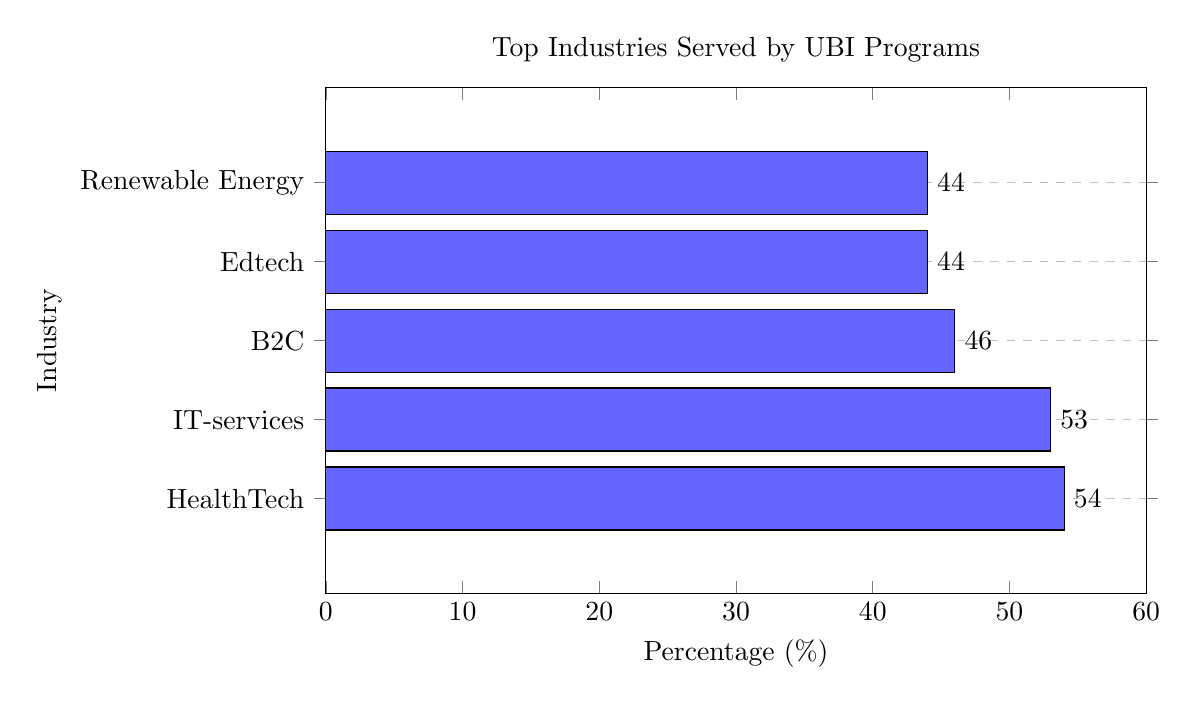
\begin{tikzpicture}
			\begin{axis}[
				title={Top Industries Served by UBI Programs},
				xlabel={Percentage (\%)},
				ylabel={Industry},
				xbar,
				xmin=0,
				xmax=60,
				width=12cm,
				height=8cm,
				bar width=0.8cm,
				nodes near coords,
				nodes near coords align={horizontal},
				ytick=data,
				yticklabels={HealthTech, IT-services, B2C, Edtech, Renewable Energy},
				ymajorgrids=true,
				grid style=dashed,
				enlarge y limits=0.3
			]
			\addplot[fill=blue!60] coordinates {
				(54,0)
				(53,1)
				(46,2)
				(44,3)
				(44,4)
			};
			\end{axis}
		\end{tikzpicture}
		\caption{Distribution of top industries served by UBI programs globally (Source: UBI Global Community Report 2023)}
		\label{fig:top_industries}
	\end{figure}

	\begin{figure}[h]
		\centering
		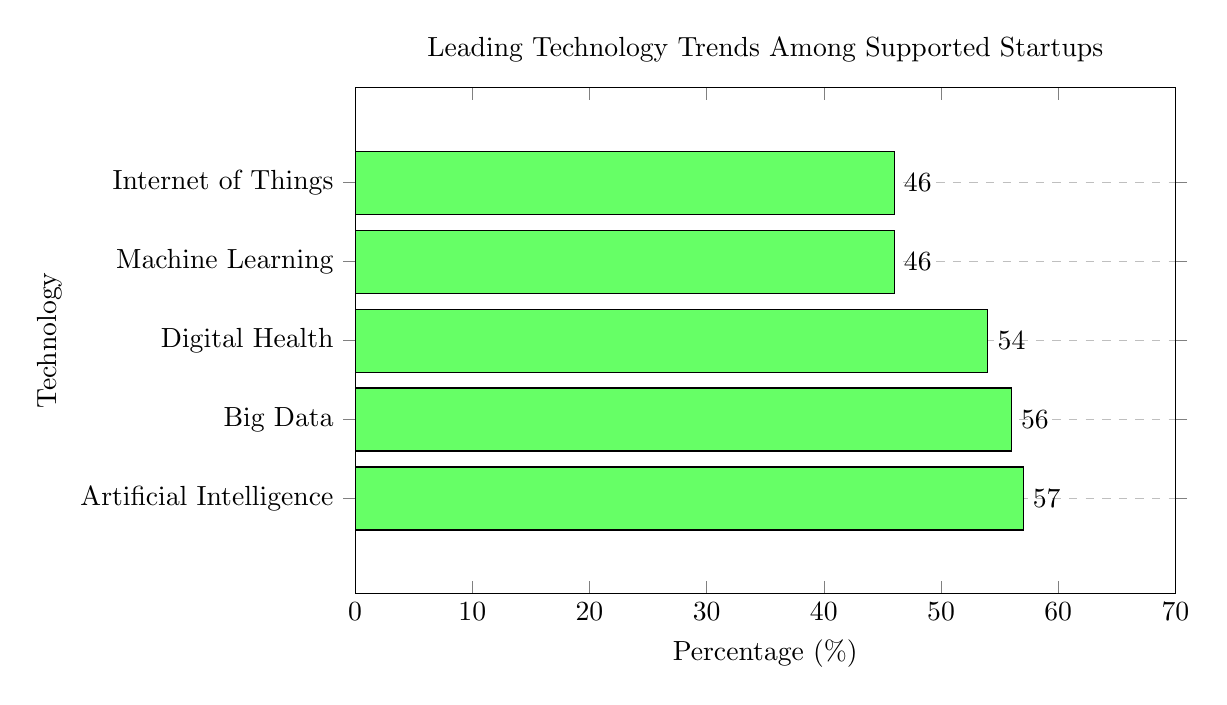
\begin{tikzpicture}
			\begin{axis}[
				title={Leading Technology Trends Among Supported Startups},
				xlabel={Percentage (\%)},
				ylabel={Technology},
				xbar,
				xmin=0,
				xmax=70,
				width=12cm,
				height=8cm,
				bar width=0.8cm,
				nodes near coords,
				nodes near coords align={horizontal},
				ytick=data,
				yticklabels={Artificial Intelligence, Big Data, Digital Health, Machine Learning, Internet of Things},
				ymajorgrids=true,
				grid style=dashed,
				enlarge y limits=0.3
			]
			\addplot[fill=green!60] coordinates {
				(57,0)
				(56,1)
				(54,2)
				(46,3)
				(46,4)
			};
			\end{axis}
		\end{tikzpicture}
		\caption{Distribution of leading technology trends among startups supported by UBI programs (Source: UBI Global Community Report 2023)}
		\label{fig:technology_trends}
	\end{figure}

	\begin{figure}[h]
		\centering
		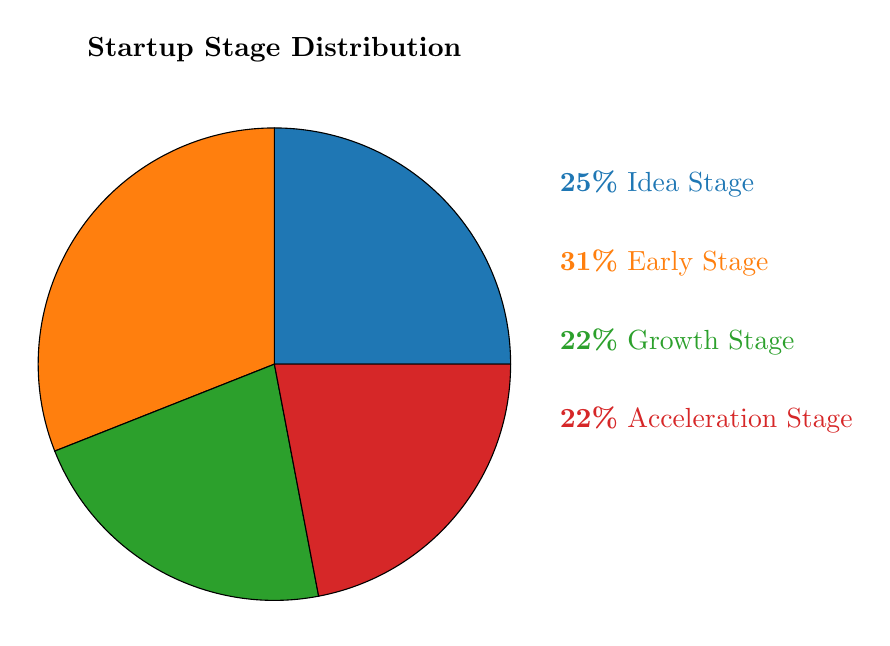
\begin{tikzpicture}
			% Define colors
			\definecolor{color1}{RGB}{31,119,180}
			\definecolor{color2}{RGB}{255,127,14}
			\definecolor{color3}{RGB}{44,160,44}
			\definecolor{color4}{RGB}{214,39,40}
			
			% Data
			\def\idea{25}
			\def\early{31}
			\def\growth{22}
			\def\accel{22}

			% Pre-calculate angles
			\pgfmathsetmacro{\angleA}{\idea*3.6}
			\pgfmathsetmacro{\angleB}{(\idea+\early)*3.6}
			\pgfmathsetmacro{\angleC}{(\idea+\early+\growth)*3.6}
			
			% Draw pie slices
			\draw[fill=color1] (0,0) -- (0:3) arc (0:\angleA:3) -- cycle;
			\draw[fill=color2] (0,0) -- (\angleA:3) arc (\angleA:\angleB:3) -- cycle;
			\draw[fill=color3] (0,0) -- (\angleB:3) arc (\angleB:\angleC:3) -- cycle;
			\draw[fill=color4] (0,0) -- (\angleC:3) arc (\angleC:360:3) -- cycle;
			
			% Add labels
			\node at (0,4) {\textbf{Startup Stage Distribution}};
			\node[above right] at (3.5,2) {\textcolor{color1}{\textbf{25\%} Idea Stage}};
			\node[above right] at (3.5,1) {\textcolor{color2}{\textbf{31\%} Early Stage}};
			\node[above right] at (3.5,0) {\textcolor{color3}{\textbf{22\%} Growth Stage}};
			\node[above right] at (3.5,-1) {\textcolor{color4}{\textbf{22\%} Acceleration Stage}};
		\end{tikzpicture}
		\caption{Distribution of startup stages supported by UBI programs (Source: UBI Global Community Report 2023)}
		\label{fig:startup_stages}
	\end{figure}

	\textbf{Change Tendency (2019-2020 to 2021-2022 and 2023):}
	From 2019-2020 to 2021-2022, UBI Global's benchmark studies show a significant reduction in the number of programs and countries included in the formal benchmarking process, with assessed programs dropping from 364 to 109 and countries from 82 to 56. This likely reflects a more stringent selection process, a focus on top-tier programs, or changes in participation rates. Despite this, the 2023 UBI Global Community report demonstrates that the broader global network of business incubators and accelerators remains extensive, with over 1,000 programs in 90+ countries. The 2023 data also highlights the increasing diversity of program types, sector focus, and regional participation, as well as the continued dominance of university-based incubators. This evolution suggests that while formal benchmarking has become more selective, the overall ecosystem is expanding and diversifying, adapting to new trends and regional needs.
	
	\begin{figure}[h]
		\centering
		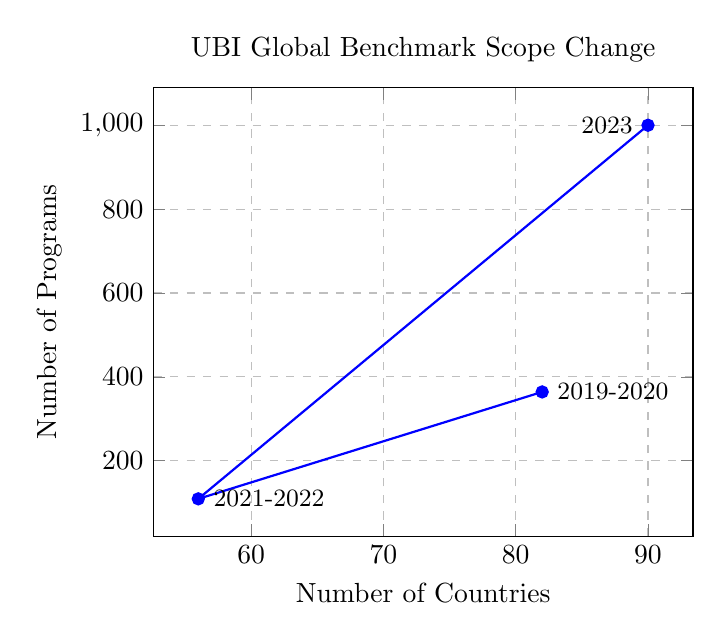
\begin{tikzpicture}
			\begin{axis}[
				title={UBI Global Benchmark Scope Change},
				xlabel={Number of Countries},
				ylabel={Number of Programs},
				ymajorgrids=true,
				xmajorgrids=true,
				grid style=dashed
			]
			
			% Add the plot with a connecting line
			\addplot[color=blue, mark=*, thick] coordinates {
				(82,364) 
				(56,109)
				(90,1000)
			};
			
			% Add labels to the points using relative positioning
			\node[right, font=\small, xshift=2pt] at (axis cs:82,364) {2019-2020};
			\node[right, font=\small, xshift=2pt] at (axis cs:56,109) {2021-2022};
			\node[left, font=\small, xshift=-2pt] at (axis cs:90,1000) {2023};
			
			\end{axis}
		\end{tikzpicture}
		\caption{Change in scope of UBI Global's benchmark studies, plotting programs vs. countries for the 2019-2020, 2021-2022, and 2023 periods.}
		\label{fig:ubi_change_tendency}
	\end{figure}
	
	\subsection{Key Performance Indicators (KPIs) and Impact Measurement Framework}
	UBI Global's comprehensive methodology for assessing program impact and performance consistently utilizes \textbf{21 Key Performance Indicators (KPIs)} across both the 2019-2020 and 2021-2022 benchmark studies \cite{ubi2019world, ubi2021world}. These KPIs are systematically grouped into three main categories, each contributing to a Program Impact and Performance Score (PIPS). All fiscal information is standardized to 2018 US dollars in the 2019-2020 report and likely similar in the 2021-2022 report for consistency.

	\begin{itemize}
		\item \textbf{Value for Ecosystem (33.3\% weight of PIPS)}: This category assesses the economic impact of the programs and their client/alumni startups, as well as their success in retaining human capital and ventures within the innovation ecosystem. It includes subcategories like "Economy Enhancement" and "Talent Retention" \cite{ubi2019world, ubi2021world}.
		\begin{itemize}
			\item \textit{Economy Enhancement} (22.2\% of PIPS) measures: Jobs created \& sustained, Sales revenue, Graduates (within 5 years), and Self-generated revenue.
			\item \textit{Talent Retention} (11.1\% of PIPS) measures: Client startups accepted (within 1 year) and Graduate retention (within 5 years).
		\end{itemize}
		\item \textbf{Value for Client Startups (33.3\% weight of PIPS)}: This category evaluates the quantity and efficiency of services provided by the programs, alongside their critical function as facilitators of community and network building. It comprises subcategories such as "Competence Development," "Access to Funds," and "Access to Network" \cite{ubi2019world, ubi2021world}.
		\begin{itemize}
			\item \textit{Competence Development} (8.9\% of PIPS) measures: Services offered and Coaching \& mentoring hours.
			\item \textit{Access to Funds} (11.1\% of PIPS) measures: Total investment attracted (within 5 years), Average investment attracted (within 5 years), and Seed funding attraction (within 1 year).
			\item \textit{Access to Network} (13.3\% of PIPS) measures: Partners, Events, and Alumni engagement.
		\end{itemize}
		\item \textbf{Value for Program (33.3\% weight of PIPS)}: This category assesses the program's success in attracting deal flow and third-party support, as well as its capacity to foster the creation of viable companies. It includes "Program Attractiveness" and "Post-Graduation Performance" subcategories \cite{ubi2019world, ubi2021world}.
		\begin{itemize}
			\item \textit{Program Attractiveness} (15.5\% of PIPS) measures: In-state applications, Out-of-state applications, and Sponsorship attraction.
			\item \textit{Post-Graduation Performance} (17.8\% of PIPS) measures: 1-year survival rate (within 10 years), 5-year survival rate (within 10 years), High-growth enterprises (within 10 years), and Qualified exits (within 10 years).
		\end{itemize}
	\end{itemize}
	While these reports detail the comprehensive KPIs utilized for benchmarking and ranking, they focus on the comparative performance of individual programs rather than providing aggregate global numerical data for the entire sample's performance across all these metrics.
	
	\subsection{Leading University Business Incubators Globally}
	UBI Global's World Rankings consistently recognize top-performing university business incubators based on their outstanding impact and value creation. The following tables show a sample of these leading incubators for the two benchmark periods.

	\begin{table}[H]
		\centering
		\caption{Leading University Business Incubators (2019-2020 Sample) \cite{ubi2019world}}
		\label{tab:leading_ubis_2019}
		\resizebox{\textwidth}{!}{%
		\begin{tabular}{|l|l|l|}
			\hline
			\textbf{Incubator} & \textbf{University} & \textbf{Country} \\
			\hline
			Chalmers Ventures & Chalmers University of Technology & Sweden \\
			The DMZ at Ryerson University & Ryerson University & Canada \\
			IPN Incubadora & University of Coimbra, Polytechnic Institute of Coimbra & Portugal \\
			PoliHub - Innovation District \& Startup Accelerator & Politecnico di Milano & Italy \\
			The SETsquared Partnership & Univ. of Bath, Bristol, Exeter, Southampton, Surrey & UK \\
			University of Toronto Entrepreneurship & University of Toronto & Canada \\
			UtrechtInc & Utrecht University, Medical Center Utrecht, UAS Utrecht & Netherlands \\
			YES!Delft & Delft University of Technology, The Hague UAS & Netherlands \\
			\hline
		\end{tabular}%
		}
	\end{table}

	\begin{table}[H]
		\centering
		\caption{Leading University Business Incubators (2021-2022 Sample) \cite{ubi2021world}}
		\label{tab:leading_ubis_2021}
		\resizebox{\textwidth}{!}{%
		\begin{tabular}{|l|l|l|}
			\hline
			\textbf{Incubator} & \textbf{University} & \textbf{Country} \\
			\hline
			Center for Technology Development (CDT) & University of Brasilia & Brazil \\
			CEI UCN & Universidad Catolica del Norte & Chile \\
			EUREKA & University of Chile & Chile \\
			Innovation, Business, and Economy Center (CIE) & Autonomous University of Baja California & Mexico \\
			King Abdullah University of Science and Technology & King Abdullah University of Science and Technology & Saudi Arabia \\
			MCB & Federal University of Campina Grande & Brazil \\
			The DMZ at Toronto Metropolitan University & Toronto Metropolitan University & Canada \\
			University of Toronto Entrepreneurship & University of Toronto & Canada \\
			UtrechtInc & Utrecht Univ., Medical Center Utrecht, UAS Utrecht, HKU Arts & Netherlands \\
			\hline
		\end{tabular}%
		}
	\end{table}
	
	These examples illustrate the continued global reach and diverse institutional affiliations of leading UBIs across different reporting periods.

	\section{Vietnam UBIs Quantitative Data}
	The Vietnamese landscape for university-based incubation programs (UBIs) and the broader startup ecosystem has undergone substantial development, marked by increasing governmental support, robust private sector engagement, and a growing entrepreneurial culture.

	\subsection{Evolution of the Startup Ecosystem and University Engagement}
	The foundational elements of Vietnam's startup ecosystem were solidified in the mid-2010s. A pivotal initiative was the Prime Minister's approval of the "National Program to Support Innovative Startup Ecosystem in Vietnam by the Year 2025," coupled with the designation of 2016 as the "Nation Year of Startup" \cite{dinh2017promoting}. This period witnessed a notable rise in entrepreneurial awareness, with the Vietnam Startup Index Report 2015/2016 indicating that the proportion of adults cognizant of business opportunities increased from 36.8\% in 2013 to 56.8\% in 2015, positioning Vietnam 9th among 60 surveyed countries \cite{dinh2017promoting}. Early university involvement manifested through the establishment of spin-off companies and business incubators. By September 2016, Vietnam operated 12 business incubators, evenly distributed between the northern (5) and southern (7) regions \cite{dinh2017promoting}. Pioneering university spin-offs, such as BK-Holdings (Hanoi University of Science and Technology) and TOPICA Education Technology Association, demonstrated the early potential of academic entrepreneurship \cite{dinh2017promoting}. These university-led ventures were crucial in fostering university-enterprise linkages and technology transfer, as exemplified by Vietnam National University's (VNU) Natural Sciences Company, which executed over 90 technology transfer contracts from 2011 to 2015 \cite{dinh2017promoting}. An internal survey in 2015 revealed that over 80\% of IT students in Ho Chi Minh City expressed a desire to initiate businesses during their studies, signaling a strong entrepreneurial inclination within the student body \cite{dinh2017promoting}.

	\begin{figure}
		\centering
		\begin{tikzpicture}
		\begin{axis}[
			xbar stacked,
			width=15cm,
			height=8cm,
			bar width=18pt,
			xmin=0, xmax=100,
			ytick=data,
			yticklabels={2023,2022,2021,2020,2019,2018,2017},
			xlabel={\%},
			legend style={at={(0.5,-0.18)}, anchor=north, legend columns=6, font=\small},
			xtick={0,20,40,60,80,100},
			tick label style={font=\small},
			ylabel={},
			title={Proportion of investment value by country},
			title style={yshift=1.5em, font=\bfseries\large},
			enlarge y limits=0.15,
			point meta=explicit,
			nodes near coords={\pgfmathprintnumber[assume math mode=true]{\pgfplotspointmeta}\%},
			nodes near coords align={center},
			nodes near coords style={font=\small, color=white,
				/pgf/number format/precision=0,
				/pgf/number format/fixed,
				/pgf/number format/fixed zerofill=false
			},
			]
		% Indonesia
		\addplot+[xbar, fill=gray!60, draw=none] coordinates {(23,0) [23] (44,1) [44] (41,2) [41] (67,3) [67] (52,4) [52] (67,5) [67] (65,6) [65]};
		% Singapore
		\addplot+[xbar, fill=gray!40, draw=none] coordinates {(56,0) [56] (27,1) [27] (33,2) [33] (14,3) [14] (19,4) [19] (0,5) [0] (19,6) [19]};
		% Malaysia
		\addplot+[xbar, fill=gray!30, draw=none] coordinates {(3,0) [3] (6,1) [6] (4,2) [4] (3,3) [3] (3,4) [3] (18,5) [18] (3,6) [3]};
		% Thailand
		\addplot+[xbar, fill=gray!20, draw=none] coordinates {(2,0) [2] (6,1) [6] (3,2) [3] (6,3) [6] (3,4) [3] (3,5) [3] (8,6) [8]};
		% Philippines
		\addplot+[xbar, fill=gray!10, draw=none] coordinates {(6,0) [6] (9,1) [9] (6,2) [6] (2,3) [2] (0,4) [0] (2,5) [2] (2,6) [2]};
		% Vietnam
		\addplot+[xbar, fill=vncolor, draw=none] coordinates {(9,0) [9] (8,1) [8] (13,2) [13] (8,3) [8] (23,4) [23] (9,5) [9] (2,6) [2]};
		\legend{Indonesia, Singapore, Malaysia, Thailand, Philippines, Vietnam}
		\end{axis}
		\end{tikzpicture}
		\caption{Proportion of investment value by country (2017--2023) \cite{vietnam_innovation_report_2024}.}
		\end{figure}
		
		\vspace{1cm}
		
		\begin{figure}
		\centering
		\begin{tikzpicture}
		\begin{axis}[
			xbar stacked,
			width=15cm,
			height=8cm,
			bar width=18pt,
			xmin=0, xmax=100,
			ytick=data,
			yticklabels={2023,2022,2021,2020,2019,2018,2017},
			xlabel={\%},
			legend style={at={(0.5,-0.18)}, anchor=north, legend columns=6, font=\small},
			xtick={0,20,40,60,80,100},
			tick label style={font=\small},
			ylabel={},
			title={Proportion of investment deals by country},
			title style={yshift=1.5em, font=\bfseries\large},
			enlarge y limits=0.15,
			point meta=explicit,
			nodes near coords={\pgfmathprintnumber[assume math mode=true]{\pgfplotspointmeta}\%},
			nodes near coords align={center},
			nodes near coords style={font=\small, color=white,
				/pgf/number format/precision=0,
				/pgf/number format/fixed,
				/pgf/number format/fixed zerofill=false
			},
			]
		% Indonesia
		\addplot+[xbar, fill=gray!60, draw=none] coordinates {(18,0) [18] (26,1) [26] (24,2) [24] (26,3) [26] (23,4) [23] (30,5) [30] (30,6) [30]};
		% Singapore
		\addplot+[xbar, fill=gray!40, draw=none] coordinates {(52,0) [52] (39,1) [39] (40,2) [40] (36,3) [36] (34,4) [34] (32,5) [32] (34,6) [34]};
		% Malaysia
		\addplot+[xbar, fill=gray!30, draw=none] coordinates {(6,0) [6] (9,1) [9] (8,2) [8] (11,3) [11] (10,4) [10] (11,5) [11] (13,6) [13]};
		% Thailand
		\addplot+[xbar, fill=gray!20, draw=none] coordinates {(3,0) [3] (4,1) [4] (4,2) [4] (5,3) [5] (9,4) [9] (8,5) [8] (10,6) [10]};
		% Philippines
		\addplot+[xbar, fill=gray!10, draw=none] coordinates {(8,0) [8] (5,1) [5] (5,2) [5] (5,3) [5] (4,4) [4] (4,5) [4] (6,6) [6]};
		% Vietnam
		\addplot+[xbar, fill=vncolor, draw=none] coordinates {(12,0) [12] (16,1) [16] (19,2) [19] (17,3) [17] (20,4) [20] (16,5) [16] (8,6) [8]};
		\legend{Indonesia, Singapore, Malaysia, Thailand, Philippines, Vietnam}
		\end{axis}
		\end{tikzpicture}
		\caption{Proportion of investment deals by country (2017--2023) \cite{vietnam_innovation_report_2024}.}
	\end{figure}

Vietnam maintains its third position in Southeast Asia in terms of deal count and returns to the third position in investment value. Singapore leads in both investment value and deal count, followed by Indonesia.

	Post-2017, the ecosystem experienced accelerated growth. The government's continued commitment is evident in initiatives like Project 844, launched in 2016 and expanded in 2021 (Decision No. 188/QD-TTg), which has extended its support to 60 provinces by 2024, with 40 localities developing financial mechanisms for startups \cite{nssc2024project}. Furthermore, Decree No. 109/2022/ND-CP specifically targets the fostering of the innovative startup ecosystem within universities \cite{nssc2024project}. The establishment of the National Innovation Center (NIC) in 2023 at Hoa Lac Hi-Tech Park serves as a central hub for promoting sustainable growth driven by science, technology, and innovation \cite{vietnam_innovation_report_2024}. By the end of 2024, Vietnam's startup ecosystem comprised over \textbf{4,000 startups}, including two unicorn companies and eleven valued over \$100 million.

	\subsection{Investment Trends and Global Standing}
	Vietnam's position in the global innovation landscape has steadily strengthened. In the Global Innovation Index 2023, Vietnam ascended to \textbf{46th position} out of 132 countries, demonstrating consistent improvement \cite{vietnam_innovation_report_2024}. The country is also recognized among the top 7 middle-income economies with the most significant innovation progress over the past decade \cite{vietnam_innovation_report_2024}. According to StartupBlink's Global Startup Ecosystem Index 2024, Vietnam rose to \textbf{56th globally} (from 58th in 2023), securing 5th place in Southeast Asia and 12th in Asia-Pacific \cite{startupblink2024, vietnamnews2024pm}.

	The venture capital landscape, while subject to global fluctuations, exhibited resilience in Vietnam. In 2023, Vietnamese startups attracted a total investment of \textbf{\$529 million} \cite{vietnam_innovation_report_2024}. This represented a 17\% decline compared to the previous year, yet it was notably milder than the 35\% global venture capital investment contraction, indicating the market's intrinsic strength \cite{vietnam_innovation_report_2024}. Vietnam maintained its third position in Southeast Asia for the volume of investment deals and successfully reclaimed the third position in total investment value within the region, trailing only Singapore and Indonesia \cite{vietnam_innovation_report_2024}.

	\begin{figure}[H]
		\centering
		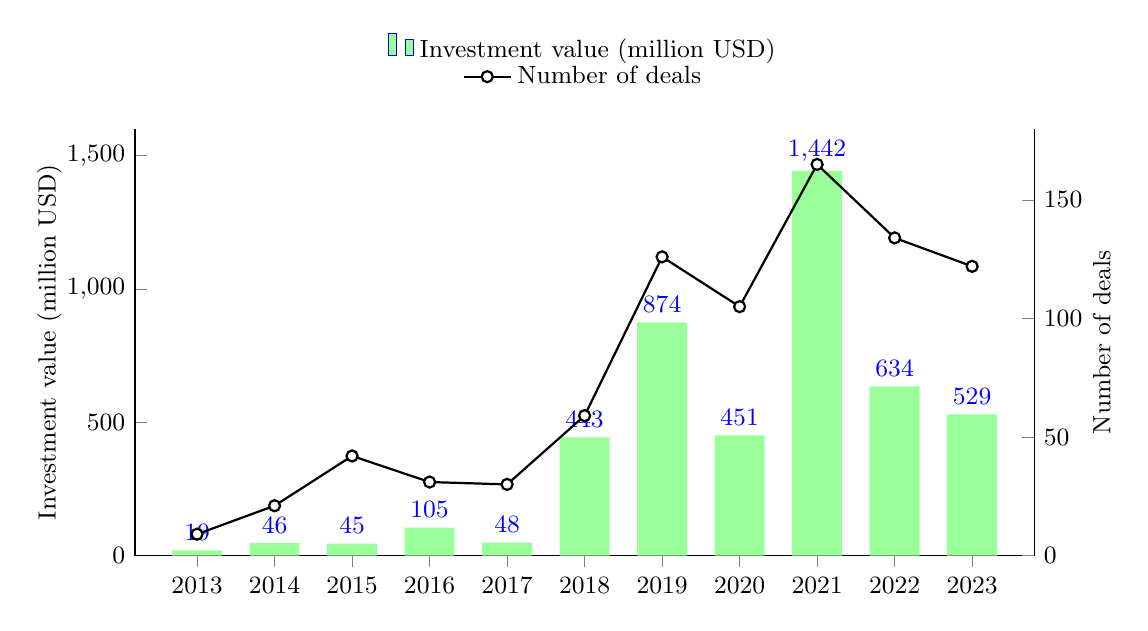
\begin{tikzpicture}
			\begin{axis}[
				width=13cm,
				height=7cm,
				ybar,
				bar width=18pt,
				ymin=0,
				ymax=1600,
				ylabel={Investment value (million USD)},
				ylabel style={yshift=-0.5em},
				axis y line*=left,
				axis x line*=bottom,
				symbolic x coords={2013,2014,2015,2016,2017,2018,2019,2020,2021,2022,2023},
				xtick=data,
				enlarge x limits=0.08,
				nodes near coords,
				nodes near coords style={above, font=\small, color=blue, text opacity=1, fill opacity=1, draw opacity=1},
				nodes near coords align={vertical},
				tick label style={font=\small},
				label style={font=\small},
				legend style={at={(0.5,1.13)}, anchor=south, legend columns=-1, font=\small, draw=none, fill=none},
			]
			% Bar plot: Investment value
			\addplot+[ybar, fill=green!40!white, draw=none] coordinates {
				(2013, 19)
				(2014, 46)
				(2015, 45)
				(2016, 105)
				(2017, 48)
				(2018, 443)
				(2019, 874)
				(2020, 451)
				(2021, 1442)
				(2022, 634)
				(2023, 529)
			};
			\addlegendentry{Investment value (million USD)}
			\end{axis}

			% Overlay line plot for number of deals
			\begin{axis}[
				width=13cm,
				height=7cm,
				ymin=0,
				ymax=180,
				axis y line*=right,
				axis x line=none,
				ylabel={Number of deals},
				ylabel style={yshift=0.3em},
				symbolic x coords={2013,2014,2015,2016,2017,2018,2019,2020,2021,2022,2023},
				xtick=data,
				enlarge x limits=0.08,
				legend style={at={(0.5,1.07)}, anchor=south, legend columns=-1, font=\small, draw=none, fill=none},
				every node near coord/.append style={font=\small, yshift=-10pt, color=black},
				tick label style={font=\small},
				label style={font=\small},
			]
			% Line plot: Number of deals
			\addplot+[
				mark=*,
				mark options={fill=white},
				color=black,
				thick
			] coordinates {
				(2013, 9)
				(2014, 21)
				(2015, 42)
				(2016, 31)
				(2017, 30)
				(2018, 59)
				(2019, 126)
				(2020, 105)
				(2021, 165)
				(2022, 134)
				(2023, 122)
			};
			\addlegendentry{Number of deals}
			\end{axis}
		\end{tikzpicture}
		\caption{Investment value and number of startup deals in Vietnam (2013--2023) \cite{vietnam_innovation_report_2024}.}
		\label{fig:vn-startup-investment}
	\end{figure}

	Sectoral investment patterns in 2023 revealed significant shifts:
	\begin{itemize}
	\item The Healthcare sector experienced a record-high investment, surging by 391\% year-over-year to become the leading invested sector \cite{vietnam_innovation_report_2024}.
	\item The Education sector also reached its highest-ever investment volume, increasing by 107\% year-over-year \cite{vietnam_innovation_report_2024}.
	\end{itemize}
	Approximately 100 funds contributed capital to Vietnamese startups in 2023, with Singaporean investors being the most active, closely followed by domestic Vietnamese investors \cite{vietnam_innovation_report_2024}. The exit market for startups is also evolving positively, marked by growth in the public market, refined stock market regulatory mechanisms, and an increasing role of local corporations in mergers and acquisitions \cite{vietnam_innovation_report_2024}.

	Despite remarkable progress, the Vietnamese university startup ecosystem continues to face challenges. These include a persistent gap between theoretical instruction and practical application in training programs, which limits hands-on experience \cite{nhandan2025startup}. Universities frequently contend with insufficient financial resources, inadequate infrastructure, and a dearth of experimental spaces and early-stage investment funds \cite{nhandan2025startup}. Furthermore, attracting international resources and securing foreign investment remains challenging, partly due to complexities in corporate restructuring requirements (e.g., establishing an offshore parent company) and regulatory ambiguities \cite{bssc2025wave, nssc2024challenges}. Startups also contend with a scarcity of suitable strategic advisors and disparities in resource access between urban and rural areas \cite{ueh2024vc}. The Prime Minister has emphasized the need for a stronger ecosystem, urging enhanced policies, particularly in finance and intellectual property, and promoting public-private partnerships to establish student startup support funds \cite{vietnamnews2025pm}.
	
\end{document}
\end{document}